In Fig.~\ref{Fig:movie}, we plot the stellar structure vs.~mass coordinate in the simulation which employs the Brown model and has $M = 1.1M_\odot$ and [Fe/H] $= -0.2$.
We limit the x-limits of the plot to the mass coordinate energy generation peak of the hydrogen burning shell on the left $m_{\rm max}$, and to $1.1 m_{\rm max}$ on the right.
An animated version of this figure is available online in the HTML version of the manuscript.

\begin{figure}[!tb]
\begin{center}
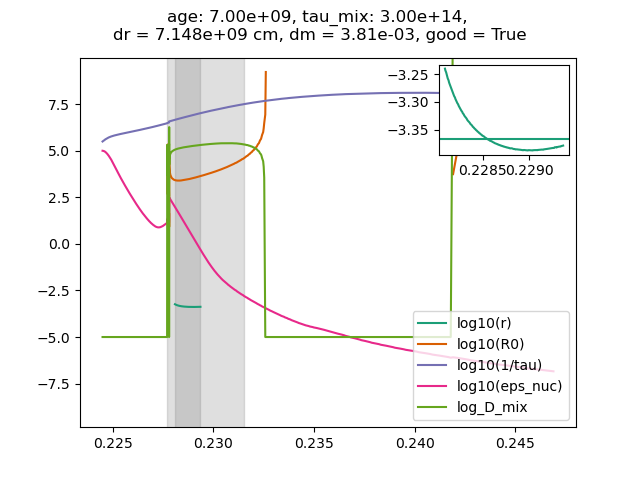
\includegraphics[width=5in]{R0_fig_003516.png}
\caption{
    We plot various stellar structure quantities (indicated in the table) vs. mass coordinate ($M / M_*$) for a $M_* = 1.1 M_\odot$ star with [Fe/H] $= -0.2$ which employs the \citet{brown_etal_2013} mixing prescription.
    We zoom in near the hydrogen burning shell, as indicated by the pink \texttt{eps\_nuc} line which shows the nuclear energy generation rate.
    The thermohaline region can be identified as the place where there is a large amount of mixing (the light green \texttt{log\_D\_mix} is large), and we shade the bulk of this region in grey.
    As described in section~\ref{sec:mesa_experiment}, we only measure $r$ over 1/3 of this region by mass, and the region over which we take this measurement is shaded in a darker grey.
    Within this region, we plot $r$ in dark green.
    A zoom-in on $log_{\rm{10}}r$ within the dark grey region is shown in the inset, and the measured value of $r$ identified by the algorithm is plotted as a dark green horizontal line.
    Additional plotted lines include $R_0$ and $1/\tau$ as described in Sec.~\ref{sec:parameterizations}.
    Various quantities are quoted in text at the top of the image, including the star's age in years, the thermohaline mixing timescale in seconds, the radial extent of the thermohaline zone in terms of both length (dr) and mass coordinate (dm), and a flag indicating that this model is identified as ``good'' by our algorithm.
    An animated version of this figure is available with the HTML version of the paper.
    }
\label{Fig:movie}
\end{center}
\end{figure}